\documentclass{beamer}

\mode<presentation> {

%\usetheme{default}
%\usetheme{AnnArbor}
%\usetheme{Antibes}
%\usetheme{Bergen}
%\usetheme{Berkeley}
%\usetheme{Berlin}
%\usetheme{Boadilla}
%\usetheme{CambridgeUS}
%\usetheme{Copenhagen}
%\usetheme{Darmstadt}
%\usetheme{Dresden}
%\usetheme{Frankfurt}
%\usetheme{Goettingen}
%\usetheme{Hannover}
%\usetheme{Ilmenau}
%\usetheme{JuanLesPins}
%\usetheme{Luebeck}
\usetheme{Madrid}
%\usetheme{Malmoe}
%\usetheme{Marburg}
%\usetheme{Montpellier}
%\usetheme{PaloAlto}
%\usetheme{Pittsburgh}
%\usetheme{Rochester}
%\usetheme{Singapore}
%\usetheme{Szeged}
%\usetheme{Warsaw}


%\usecolortheme{albatross}
%\usecolortheme{beaver}
%\usecolortheme{beetle}
%\usecolortheme{crane}
%\usecolortheme{dolphin}
%\usecolortheme{dove}
%\usecolortheme{fly}
%\usecolortheme{lily}
%\usecolortheme{orchid}
%\usecolortheme{rose}
%\usecolortheme{seagull}
%\usecolortheme{seahorse}
%\usecolortheme{whale}
%\usecolortheme{wolverine}

%\setbeamertemplate{footline} % To remove the footer line in all slides uncomment this line
%\setbeamertemplate{footline}[page number] % To replace the footer line in all slides with a simple slide count uncomment this line

%\setbeamertemplate{navigation symbols}{} % To remove the navigation symbols from the bottom of all slides uncomment this line
}

\usepackage{graphicx} % Allows including images
\usepackage{booktabs} % Allows the use of \toprule, \midrule and \bottomrule in tables
\usepackage{amsfonts}
\usepackage{mathrsfs}
\usepackage{amsmath,amssymb,graphicx}

\newcommand{\verbatimfont}[1]{\renewcommand{\verbatim@font}{\ttfamily#1}} % small verbatim

%----------------------------------------------------------------------------------------
%	TITLE PAGE
%----------------------------------------------------------------------------------------

\title["1.3"]{1.3: Some Simple Time Series Models} 

\author{Taylor} 
\institute[UVA] 
{
University of Virginia \\
\medskip
\textit{} 
}
\date{} 

\begin{document}
%----------------------------------------------------------------------------------------

\begin{frame}
\titlepage 
\end{frame}
%----------------------------------------------------------------------------------------

\begin{frame}
\frametitle{Definition}

\begin{block}{defn}
A {\bf time series model} for the oberved data $x_1, x_2, \ldots, x_T$, is a specification of the joint distributions of a sequence of random variables $X_1, \ldots, X_T$, of which $x_1, \ldots, x_T$ are postulated to be a realization.
\end{block}


It describes {\bf all} cumulative distribution functions (CDFs) you can think of:
\[
F_{X_{i_1}, \ldots, X_{i_n}}(x_{i_1}, \ldots, x_{i_n}) = P(X_{i_1} \le x_{i_1}, \ldots, X_{i_n} \le x_{i_n})
\] for any $n$, and $i_1 < i_2 < \cdots < i_n$.
\newline

It completely defines all behavior.


\end{frame}

%----------------------------------------------------------------------------------------

\begin{frame}
\frametitle{Common Practice}

Usually we just look at {\bf second order properties} of a time series. 
\newline

This means we look at the 
{\bf first-order} means $E[X_t]$, and the {\bf second-order} expected products (building blocks of covariances) $E[X_tX_{t+h}]$, for any $t \in T_0$, and $h=1,2,\ldots$.
\newline

Sometimes this is sufficient. Sometimes, for complicated time series, it is not. What follows are a few simple models where it is sufficient to just know the second-order properties. In other words, where knowing the means and variances fully specifies a model.

\end{frame}

%----------------------------------------------------------------------------------------

\begin{frame}
\frametitle{Example 1: IID Noise}

$X_1, \ldots, X_T$ are {\bf iid  noise} if they are 

\begin{enumerate}
\item {\bf independent}:
  \[
    F_{X_{1}, \ldots, X_{T}}(x_{1}, \ldots, x_{n}) = F_{X_{1}}(x_1) \times  \cdots, F_{X_{T}}(x_{T}),
  \] for all $\{x_i\}$ and
\item {\bf identical}: 
  \[
    F_{X_i}(x_i) = F(x_i)
  \]for all $i$, and
\item {\bf noise} 
  \[
  E[X_t] = 0
  \]
  for all $t$
\end{enumerate}


\end{frame}

%----------------------------------------------------------------------------------------

\begin{frame}[fragile]
\frametitle{Example 1: IID Noise}

IID noise has no trend, no seasonality, and no pattern in general. Sometimes they are assumed be all be {\bf Normally distributed}. Or sometimes they are assumed to be iid {\bf Bernoulli random variables} (a Binomial random variable when $n=1$).
\newline

The outcomes of a Bernoulli rv are usually coded as $1$ and $0$. However, to get a mean of $0$, we assume the outcomes are coded as $1$ and $-1$, and we assume $p=.5$.
\newline

\begin{verbatim}
plot(sample(x=c(1,-1), size=50, 
            replace=T, prob=c(.5,.5)), type = "b", 
            ylab = "xt")
\end{verbatim}
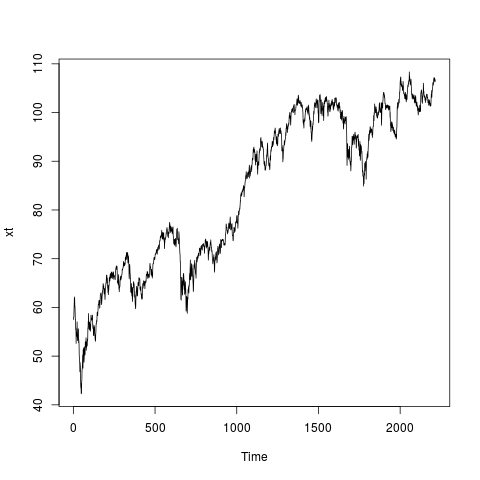
\includegraphics[width=40mm]{/home/taylor/UVa/all_teaching/4170_slides/1/1.3/pics/Rplot}
\end{frame}

%----------------------------------------------------------------------------------------

\begin{frame}[fragile]
\frametitle{Example 2: Random Walk}

A {\bf (simple symmetric) random walk} is obtained by summing iid noise. For each $t = 1, 2, \ldots$
\[
S_t = X_1 + X_2 + \cdots X_t = \sum_{i=1}^t X_i.
\]
Usually it's convention to set $S_0 = 0$ with probability $1$.

\begin{verbatim}
plot(cumsum(sample(x=c(1,-1), size=50, replace=T, 
     prob=c(.5,.5))), type = "l", ylab = "st")
\end{verbatim}
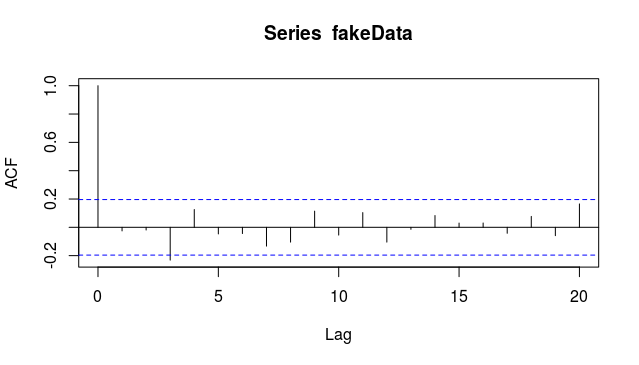
\includegraphics[width=40mm]{/home/taylor/UVa/all_teaching/4170_slides/1/1.3/pics/Rplot01}
\end{frame}

%----------------------------------------------------------------------------------------

\begin{frame}[fragile]
\frametitle{Example 3: Adding a Deterministic Trend}

\[
X_t = m_t + Y_t
\]

\begin{enumerate}
\item $X_t$: object of interest
\item $m_t$: trend that we try to estimate
\item $Y_t$: iid noise
\end{enumerate}
\end{frame}
%----------------------------------------------------------------------------------------

\begin{frame}[fragile]
\frametitle{Example 3: Adding a Deterministic Trend}

Example 1.3.4: A polynomial trend. Assume $m_t = a_0 + a_1t + a_2 t^2$, for some unknown $a_0$, $a_1$ and $a_2$. See 1.3.R file.\\

\begin{center}
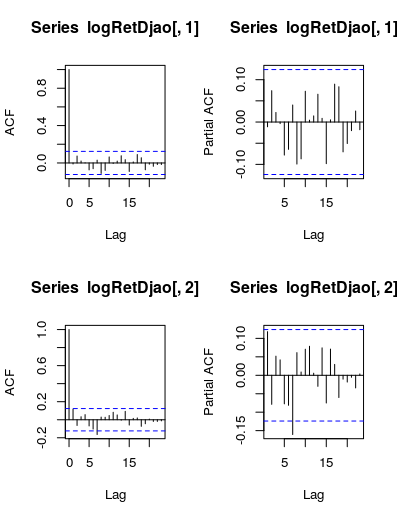
\includegraphics[width=100mm]{/home/taylor/UVa/all_teaching/4170_slides/1/1.3/pics/Rplot02}
\end{center}

\end{frame}

%----------------------------------------------------------------------------------------

\begin{frame}[fragile]
\frametitle{Example 3: Adding a Deterministic Trend}

\begin{verbatim}
> summary(fitMod)

Call:
lm(formula = population ~ t + I(t^2), data = popData)

Residuals:
     Min       1Q   Median       3Q      Max 
-6947521  -358167   436285  1481410  3391761 

Coefficients:
            Estimate Std. Error t value Pr(>|t|)    
(Intercept)  6957920    1998526   3.482  0.00266 ** 
t           -2159870     418437  -5.162 6.55e-05 ***
I(t^2)        650634      18472  35.223  < 2e-16 ***
---
Signif. codes:  0 ‘***’ 0.001 ‘**’ 0.01 ‘*’ 0.05 ‘.’ 0.1 ‘ ’ 1

Residual standard error: 2767000 on 18 degrees of freedom
Multiple R-squared:  0.9989,	Adjusted R-squared:  0.9988 
F-statistic:  8050 on 2 and 18 DF,  p-value: < 2.2e-16
\end{verbatim}
\end{frame}

%----------------------------------------------------------------------------------------

\begin{frame}[fragile]
\frametitle{Example 3: Adding a Deterministic Trend}

Example 1.3.5: assume $m_t = a_0 + a_1t$, for some unknown $a_0$ and $a_1$. See 1.3.R file.\\

\begin{center}
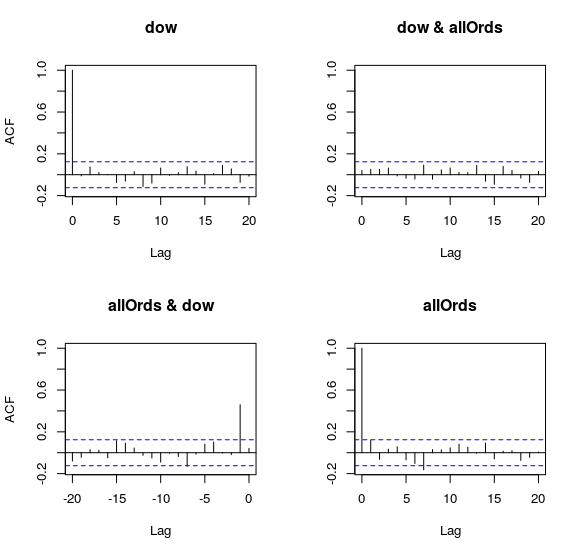
\includegraphics[width=60mm]{/home/taylor/UVa/all_teaching/4170_slides/1/1.3/pics/Rplot03}
\end{center}
\begin{center}
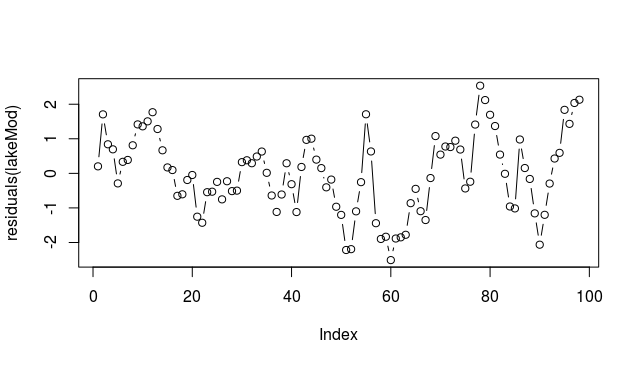
\includegraphics[width=60mm]{/home/taylor/UVa/all_teaching/4170_slides/1/1.3/pics/Rplot04}
\end{center}
\end{frame}
%----------------------------------------------------------------------------------------

\begin{frame}[fragile]
\frametitle{Example 4: Adding a Deterministic Trend}

Harmonic Regression. Adding a seasonal trend.
\[
X_t = s_t + Y_t
\]

\begin{enumerate}
\item $X_t$: object of interest
\item $s_t$: periodic function that we try to estimate
\item $Y_t$: iid noise
\end{enumerate}
\end{frame}

%----------------------------------------------------------------------------------------

\begin{frame}[fragile]
\frametitle{Example 4: Adding a Deterministic Trend}

Some background first:
\begin{enumerate}
\item {\bf period:} units: time / 1 cycle
\item {\bf frequency:} $f$, units: cycles / 1 time
\item frequency and period are reciprocals
\item Units of $2\pi f $ are radians / 1 time
\item Units of $2 \pi f t$ are radians
\item Sometimes people write $\lambda = 2 \pi f$ (angular frequency)
\item Angle-Sum Trig Identity: $\cos(a + b) = \cos(a) \cos(b) - \sin(a) \sin(b)$
\item Think unit circle: $\cos(0) = \cos(2\pi) = 1$, etc.
\end{enumerate}
\end{frame}

%----------------------------------------------------------------------------------------

\begin{frame}[fragile]
\frametitle{Example 4: Adding a Deterministic Trend}

\begin{align*}
s_t &= a_0 + \sum_{j=1}^k A_j \cos(2\pi f_j t + \phi_j) && \text{amps and phase} \\
&= a_0 + \sum_{j=1}^k A_j \cos(2\pi f_j t) \cos( \phi_j) - A_j\sin(2 \pi f_j t) \sin(\phi_j)  \\
&= a_0 + \sum_{j =1}^k \left[a_j\cos(2\pi f_j t) + b_j\sin(2\pi f_j t) \right] && \text{use this one}
\end{align*}

Known frequencies: $f_1, \ldots, f_k$\\
To be estimated: $a_0, a_1, \ldots, a_k, b_1, \ldots, b_k$
\end{frame}

%----------------------------------------------------------------------------------------

\begin{frame}[fragile]
\frametitle{Example 4: Adding a Deterministic Trend}

\begin{center}
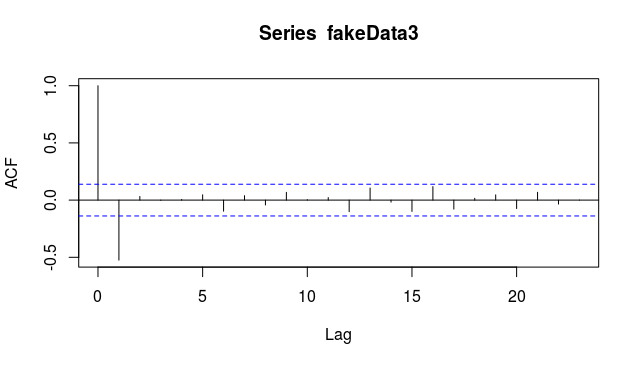
\includegraphics[width=100mm]{/home/taylor/UVa/all_teaching/4170_slides/1/1.3/pics/Rplot05}
\end{center}
\end{frame}

\end{document} 